\documentclass[we,final,11pt,oneside,openany]{uantwerpenbamathesis}
% \documentclass[we,a4paper,11pt,twoside,openright]{uantwerpenbamathesis}

\usepackage[english]{babel}

%% this is just for some dummy text, please remove in your copy
\usepackage{kantlipsum}
\usepackage{natbib}
\usepackage[linesnumbered,ruled,vlined]{algorithm2e}
\usepackage{listings}
\usepackage{xcolor}
\usepackage{amssymb}
\newcommand{\algorithmfootnote}[1]{\leavevmode\rlap{\footnotesize #1}\par}
\usepackage{todonotes}
\usepackage{float}
\usepackage{subcaption}
\usepackage{dirtree}
\usepackage{mwe}
\usepackage{wrapfig}

%% this package allows to generate a PDF with clickable links
\usepackage[backref,hyperindex=true,pagebackref=true]{hyperref}

\usepackage{cleveref}
%% as an example - loading some fonts, feel free to change
\usepackage{mathptmx}
\iftutex
%% Just an example of font-scheme: this is in no way a recommended font
%% scheme!
\usepackage{fontspec}
\setmainfont
[UprightFont = *,
 BoldFont = *b,
 ItalicFont = *i,
 BoldItalicFont = *z,
]
{calibri}
\usepackage{sansmathaccent}
\fi

\lstdefinestyle{bashstyle}{
  language=bash,
  basicstyle=\ttfamily\small,
  backgroundcolor=\color{gray!10},
  frame=single,
  rulecolor=\color{gray!60},
  frameround=tttt,
  keywordstyle=\color{blue},
  commentstyle=\color{green!60!black}\itshape,
  stringstyle=\color{orange},
  showstringspaces=false,
  breaklines=true,
  columns=fullflexible,
  captionpos=b,
  keywords={\$}
}

\lstdefinestyle{pythonstyle}{
  language=Python,
  basicstyle=\ttfamily\small,
  backgroundcolor=\color{gray!10},
  frame=single,
  rulecolor=\color{gray!60},
  frameround=tttt,
  keywordstyle=\color{blue},
  commentstyle=\color{green!60!black}\itshape,
  stringstyle=\color{green!60!black},
  showstringspaces=false,
  breaklines=true,
  columns=fullflexible,
  captionpos=b
}

\bamadegree{we-en-ma-em}

\title{Provide a title}

\author{Inte Vleminckx}
\supervisor{prof. dr. H. Vangheluwe}{UAntwerpen}
\supervisor{R. Mittal, Doctoral Fellow}{UAntwerpen}

\academicyear{2024 - 2025}

%% you can specify a company logo
%%\companylogo{\includegraphics[width=4.5cm,height=2.5cm,keepaspectratio]{companylogo.jpg}}

\begin{document}

%% creates the title page, remove if you don't want any
\maketitle

%% causes the first pages to be roman numbered
\frontmatter

%% sets the table of contents (automatically for you)
\tableofcontents

%% changes the numbering system to arabic and restart from 1
\mainmatter

% %%%%%%%%%%%%%%%%%%%%%%%%%%%%%%%%%%%%%%%%%%%%%%%%%%%%%%%%%%% %
% %%%%%%%%%%%%%%%%%%%%%%%%%%%%%%%%%%%%%%%%%%%%%%%%%%%%%%%%%%% %
% %%%%%%%%%%%%%%%%%%%%%%%%%%%%%%%%%%%%%%%%%%%%%%%%%%%%%%%%%%% %
\chapter{Introduction}
\label{ch:introduction}

The development of products in the heating, ventilation, and air conditioning (HVAC) industry presents significant challenges in testing and validation.
Building physical prototypes for every design iteration is often costly and time-consuming.
A promising alternative is to model the most expensive or complex components in a virtual environment, enabling early testing without full-scale prototypes.
This approach allows the evaluation of critical subsystems, particularly the control software that regulates HVAC systems.

In this study, we investigate how to test the control loop of a heating and ventilation system by modeling all physical elements—such as the valve, the actuator controlling the valve, the flow sensor, the pipe network, and the pressure pump that generates the fluid flow.
The control loop, which determines the actuator setpoint based on the flow sensor measurements, will interact with the virtual model using co-simulation techniques.
To assess the feasibility and performance of this approach, we compare two testing strategies: Software-in-the-Loop (SiL), and Hardware-in-the-Loop (HiL).
In SiL testing, the model interacts with a compiled version of the control loop running on a separate system, with all connections established virtually.
In HiL testing, the model runs on one system while the control loop is executed on the actual embedded hardware used in the real setup, with physical connections between the two.

Our methodology proceeds in stages.
First, we develop a simple flow circuit in Modelica to demonstrate basic co-simulation capabilities.
Using this model, we investigate how to integrate it with SiL and HiL environments.
Once this foundation is established, we expand the Modelica component library with more detailed and realistic system elements.
Finally, we construct an advanced flow circuit model and benchmark SiL results against HiL results to evaluate performance differences and validate the modeling approach.

\todo{Inte: add what can be expected in each upcomming section in one sentece.}


% %%%%%%%%%%%%%%%%%%%%%%%%%%%%%%%%%%%%%%%%%%%%%%%%%%%%%%%%%%% %
% %%%%%%%%%%%%%%%%%%%%%%%%%%%%%%%%%%%%%%%%%%%%%%%%%%%%%%%%%%% %
% %%%%%%%%%%%%%%%%%%%%%%%%%%%%%%%%%%%%%%%%%%%%%%%%%%%%%%%%%%% %
\chapter{The First Steps}
\label{ch:the-first-steps}

To address the problem at hand, we must first establish a clear understanding of the overall problem statement.
As outlined in the introduction, our goal is to test the control loop of a heating and ventilation system by modeling all physical elements and allowing the control loop to interact with this model.
To achieve this, we need to define, as simply as possible, what the model requires as input from the control loop and what the control loop requires as input from the model, without yet considering detailed configuration parameters of the individual physical components.
With this understanding in place, we can represent the interaction between the control loop and the model using the following diagram:

\begin{figure}[h!]
    \centering
    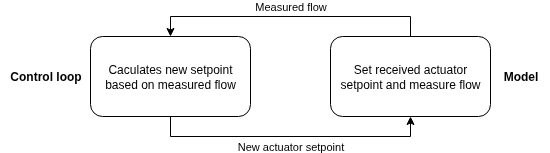
\includegraphics[width=0.6\linewidth]{Images/generated/simple-representation}
    \caption{Simple represention of interaction between control loop and model}
    \label{fig:simple-representation}
\end{figure}

Next, we provide a more detailed explanation of the process illustrated in \autoref{fig:simple-representation}.
In this setup, the control loop receives a target flow setpoint.
Although the source of this setpoint is not relevant to our study, it defines the desired flow rate in the circuit.
To achieve this flow rate, the control loop calculates an actuator setpoint, which adjusts the valve opening to provide the required flow.
In order to perform this calculation, the control loop must receive feedback from the model in the form of the measured flow in the circuit.
By comparing the measured flow to the target flow, the control loop can determine the necessary actuator setpoint and adjust the valve position accordingly.

With this simplified setup, we can construct a Modelica model that accepts one real-valued input and produces one real-valued output—the actuator setpoint and the measured flow, respectively.
For testing purposes, we can initially provide fixed output values from the model to the control loop to observe how the actuator setpoint evolves over time.
To enable full co-simulation, we must also determine how to establish interaction between the Modelica model and the control loop.
The workflow for this process is as follows:
\begin{enumerate}
    \item Develop a simple Modelica model.
    \item Investigate how the compiled control loop can be accessed and controlled using Python.
    \item Integrate the Modelica model into the Python code so that the control loop can exchange data with the model in real time.
\end{enumerate}

\newpage

\section{A Simple Modelica Model}
\label{sec:a-simple-modelica-model}

A very simple Modelica model can be represented as shown in \autoref{fig:simple-modelica-model}.
\begin{figure}[h!]
    \centering
    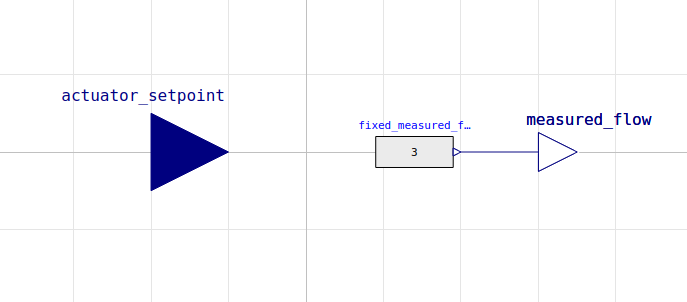
\includegraphics[width=0.6\linewidth]{Images/modelica/simple-representation}
    \caption{A simplified model representatino}
    \label{fig:simple-modelica-model}
\end{figure}

This model accepts an actuator setpoint as input and produces a measured flow as output, which is currently fixed at a value of 3 for testing purposes.

\section{Interaction With The Control Loop}
\label{sec:interaction-with-the-control-loop}

The first step in enabling interaction with the control loop is to compile the common platform—containing the control loop—into an executable.
This common platform is implemented in C and is compiled using CMake.
Due to privacy regulations of the company related to this study, the source code of the common platform cannot be shared.

Once the executable is available, the next step is to establish a method for interacting with the common platform.
There are two primary communication interfaces used by the platform:

\begin{enumerate}
    \item A Flow Sensor Board (FSB), which emulates the behavior of a real flow sensor using a UART connection.
    \item A Modbus interface, which allows reading registers from the embedded control board using a TCP connection.
\end{enumerate}

In the case of Software-in-the-Loop (SiL) testing, the common platform is executed locally.
A mock Modbus connection is created to replicate the behavior of a physical Modbus link to an embedded board.
To keep the discussion focused, we first consider only the SiL setup.
A schematic representation of this communication is shown in \autoref{fig:common-platform-communication}.

\begin{figure}[h!]
    \centering
    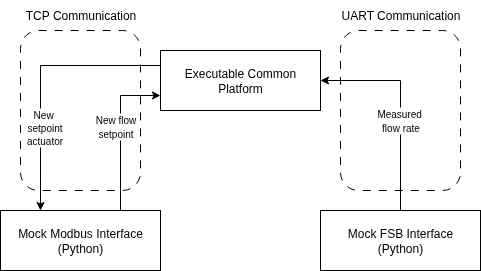
\includegraphics[width=0.6\linewidth]{Images/generated/common-platform-communication}
    \caption{Overview communication with common platform}
    \label{fig:common-platform-communication}
\end{figure}

To enable this interaction, we must first create virtual serial ports that allow communication with the common platform.
This can be achieved using the following commands:

\begin{lstlisting}[style=bashstyle, caption={Creating virtual ports for communication}]
$ sudo socat -d -d pty,link=/dev/ttyV1,raw,echo=0 pty,link=/dev/ttyV2,raw,echo=0
$ sudo chmod 777 /dev/ttyV1 && sudo chmod 777 /dev/ttyV2 && \
sudo socat -d -d -u OPEN:/dev/ttyV1,raw tcp:localhost:8888,reuseaddr
\end{lstlisting}

\newpage

This configuration uses socat to create a pair of virtual serial ports and forward data through a TCP socket.
First, it establishes two pseudo-terminal devices—/dev/ttyV1 and /dev/ttyV2—which function as the two ends of a virtual null-modem cable: any data written to one port immediately appears on the other.
Next, their permissions are updated to allow unrestricted access, and a second socat process forwards all data received on /dev/ttyV1 to a TCP connection on port 8888.

The final step is to connect to the virtual ports from Python, enabling direct interaction with the common platform through Python code.

To achieve this, we use two Python modules:
\begin{enumerate}
    \item The serial module.
    \item The ModbusTcpClient module from the pymodbus.client library.
\end{enumerate}

The serial module is used to implement the Flow Sensor Board (FSB) mock.
For this purpose, we create a PeriodicPacket class that encapsulates all the data expected by the common platform from a real FSB.
This packet is serialized into a byte format compatible with the common platform and transmitted over the serial connection via /dev/ttyV2.

The ModbusTcpClient module is used to implement the Modbus mock.
This allows us to read and write registers that correspond to specific data points within the common platform.
The Modbus client runs on localhost with port 8080.

Using this setup, we can send new flow measurements to the common platform by updating the PeriodicPacket and transmitting it over the serial connection.
Additionally, by accessing the appropriate registers, we can read the actuator setpoint calculated by the common platform and write new flow setpoints directly into the system.

\newpage

\section{Complete Integration}
\label{sec:complete-integration}

To complete the integration, we must also interact with the Modelica model developed earlier.

The first step is to export the Modelica model so that it can be integrated into Python.
This is achieved by exporting the model as a Functional Mock-up Unit (FMU).
Since we intend to perform co-simulation, the FMU export must explicitly be configured for co-simulation mode rather than model-exchange mode.

Several Python libraries support FMU-based simulation, but not all of them allow for co-simulation with externally controlled simulation steps.
Step control is essential because we need to dynamically update the model inputs and retrieve outputs during execution, ensuring synchronization with the common platform.
For this reason, we select the fmpy library, which provides full co-simulation capabilities and fine-grained step control.

With this functionality in place, the final task is to design a simulation loop that integrates all components, ensuring seamless data exchange between the Modelica model and the common platform.
Before proceeding to implementation, we present a schematic diagram in \autoref{fig:full-communication} summarizing the complete interaction setup.
This diagram highlights the data flow between all components and clarifies which elements produce or consume specific signals.

\begin{figure}[h!]
    \centering
    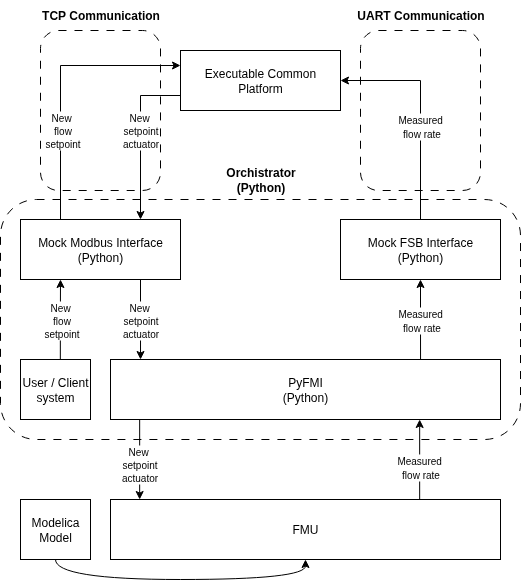
\includegraphics[width=0.6\linewidth]{Images/generated/full-communication.drawio}
    \caption{Total interaction overview between all components}
    \label{fig:full-communication}
\end{figure}

We observe that this diagram extends \autoref{fig:common-platform-communication}, with the orchestrator managing the communication between the common platform and the FMU.
The simulation loop, capturing all interactions, is implemented as follows:

\newpage

\begin{lstlisting}[style=pythonstyle, caption={Simulation loop}]
def run(self):
    performed_step = True
    self._modbus.set_setpoint_flow(0.0)

    while performed_step:
        time = self._model.current_time

        # Update measured flow
        m_flow = self._model.get_measured_flow()
        self._fsb.update_flow(m_flow)

        # Update model with new setpoint
        s_motor = self._modbus.get_setpoint_motor()
        self._model.set_setpoint_motor(s_motor)

        self._update_trace(time, m_flow, s_flow, s_motor)

        # Perform a step in the model
        performed_step = self._model.perform_step()
\end{lstlisting}

For testing purposes, the simulation loop is deliberately kept simple.
First, the measured flow is retrieved from the Modelica model and passed to the FSB, which transmits the corresponding packet to the common platform.
Next, the motor setpoint is read from its Modbus register and sent back to the Modelica model.
A trace of the key variables is recorded to enable visualization, and finally, the model performs a single simulation step.

To verify correct operation, two test cases are executed: one with the flow setpoint s\_flow = 2.0 and another with s\_flow = 0.0.
The objective is to confirm that the common platform’s control loop generates different motor positions depending on whether the flow setpoint is above or below the fixed measured flow value provided by the Modelica model (which is constant at 1.0 in this scenario).

\begin{figure}[h!]
    \begin{subfigure}{.5\textwidth}
        \centering
        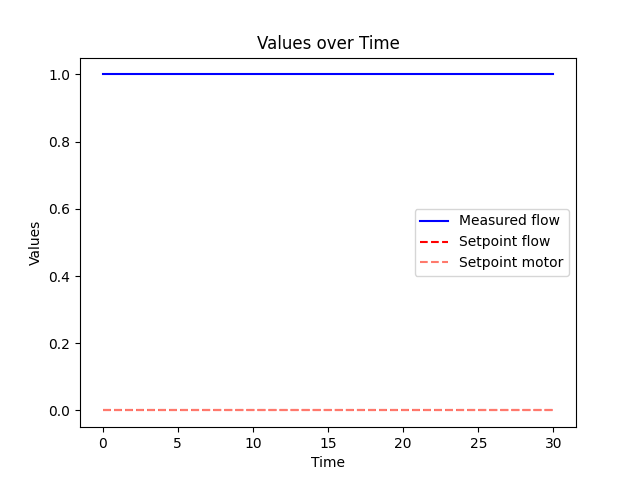
\includegraphics[width=.8\linewidth]{Images/simulations/simple_simulation_0}
        \caption{Simple simulation with s\_flow = 0.0}
        \label{fig:simple-sim-0}
    \end{subfigure}%
    \begin{subfigure}{.5\textwidth}
        \centering
        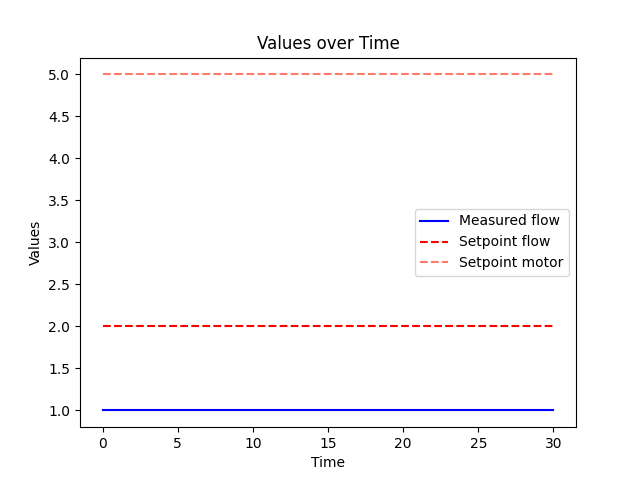
\includegraphics[width=.8\linewidth]{Images/simulations/simple_simulation_2}
        \caption{Simple simulation with s\_flow = 2.0}
        \label{fig:simple-sim-2}
    \end{subfigure}
\end{figure}

As shown in \autoref{fig:simple-sim-0}, the motor setpoint is calculated as 0 when s\_flow = 0, whereas in \autoref{fig:simple-sim-2}, the motor setpoint is 5 when s\_flow = 2.0, both evaluated against a fixed measured flow of 1.0.
These results confirm that the control loop correctly receives the measured flow and computes the motor setpoint accordingly.

This demonstrates that the minimal setup functions as intended: all components successfully interact with one another.
With this validation in place, the next step is to extend the Modelica components to simulate a complete flow circuit and enhance the Python code to support the expanded system.

% %%%%%%%%%%%%%%%%%%%%%%%%%%%%%%%%%%%%%%%%%%%%%%%%%%%%%%%%%%% %
% %%%%%%%%%%%%%%%%%%%%%%%%%%%%%%%%%%%%%%%%%%%%%%%%%%%%%%%%%%% %
% %%%%%%%%%%%%%%%%%%%%%%%%%%%%%%%%%%%%%%%%%%%%%%%%%%%%%%%%%%% %
\chapter{Modelica Library Overview}
\label{ch:modelica-library-overview}

In this study, a flow circuit consists of several interconnected components, including a pressure pump, pipes with bends, and the primary unit, Dynamx, which integrates a valve, a flow sensor, and a linear actuator to regulate the valve position.
To facilitate the construction of such flow circuits, all components must be modeled in a modular and user-friendly way.
For this purpose, additional packages have been introduced into our Modelica library, including a configuration block and a set of base component models.
An overview of the most relevant packages and models in the library is provided in the following sections.


\section{Configurations}
\label{sec:configurations}

\subsection{Configuration}
\label{subsec:configuration}

The Configuration model must be included in the flow model and should always be named config (this is also the default name).
This model defines the parameters used to configure the actuator, Dynamx, and valve components.
By using this configuration model, parameter values for all components in the flow model can be conveniently adjusted directly from the Python code.
For this reason, the name config is important, as it allows the Python interface to reliably locate the configuration model.
We will discuss this in more detail in \autoref{ch:python-interface}.

\begin{table}[h!]
\centering
\begin{tabular}{|lcl|}
\hline
\multicolumn{1}{|l|}{\textbf{Parameter}}     & \multicolumn{1}{c|}{\textbf{Unit}} & \textbf{Description}                                     \\ \hline
\multicolumn{3}{|l|}{\textit{Dynamx settings - Actuator}}                                                                                    \\ \hline
\multicolumn{1}{|l|}{min\_motor\_position}   & \multicolumn{1}{c|}{-}             & The minimum position of the actuator                     \\ \hline
\multicolumn{1}{|l|}{max\_motor\_position}   & \multicolumn{1}{c|}{-}             & The maximum position of the actuator                     \\ \hline
\multicolumn{1}{|l|}{start\_motor\_position} & \multicolumn{1}{c|}{-}             & The start position of the actuator                       \\ \hline
\multicolumn{1}{|l|}{total\_opening\_time}   & \multicolumn{1}{c|}{s}             & Time to reach maximum position from its minimum          \\ \hline
\multicolumn{1}{|l|}{total\_closing\_time}   & \multicolumn{1}{c|}{s}             & Time to reach minimum position from its maximum          \\ \hline
\multicolumn{3}{|l|}{\textit{Dynamx settings - Valve}}                                                                                       \\ \hline
\multicolumn{1}{|l|}{valve\_diameter}        & \multicolumn{1}{c|}{mm}            & Diameter of the pipe of the valve                        \\ \hline
\multicolumn{1}{|l|}{max\_valve\_flow\_rate} & \multicolumn{1}{c|}{kg/s}          & Maximun flow rate of the valve at full opening           \\ \hline
\multicolumn{3}{|l|}{\textit{Dynamx settings - Valve (if equal percentage)}}                                                                 \\ \hline
\multicolumn{1}{|l|}{leakage}                & \multicolumn{1}{c|}{l}             & Valve leakage                                            \\ \hline
\multicolumn{1}{|l|}{R}                      & \multicolumn{1}{c|}{-}             & Reangeability, between 50 and 100 typically              \\ \hline
\multicolumn{1}{|l|}{delta0}                 & \multicolumn{1}{c|}{-}             & Range of significant deviation from equal percentage law \\ \hline
\multicolumn{1}{|l|}{deltaM}                 & \multicolumn{1}{c|}{-}             & Fraction of nominal flow rate where linearization starts \\ \hline
\multicolumn{3}{|l|}{\textit{Pump settings}}                                                                                                 \\ \hline
\multicolumn{1}{|l|}{pump\_pressure}         & \multicolumn{1}{c|}{pa}            & The pressure of the pump                                 \\ \hline
\end{tabular}
\caption{All configuration parameters}
\label{tab:config-table}
\end{table}

\newpage

\autoref{tab:config-table} lists all configurable parameters for the different components.
Most of these parameters are overwritten when setting up the simulation in Python.
The table also contains a section that applies only when an equal percentage valve is used.
This distinction arises because linear valves and equal percentage valves require different configuration parameters.
When creating the Modelica model, you can select a checkbox to make these parameters editable.
Note, however, that these valve-specific parameters cannot be modified through Python.
Default values are provided, but any changes must be made directly in the Modelica model itself.

\section{Actuators}
\label{sec:actuators}

\subsection{Actuator}
\label{subsec:actuators}

\begin{wrapfigure}{R}{0.15\textwidth}
    \centering
    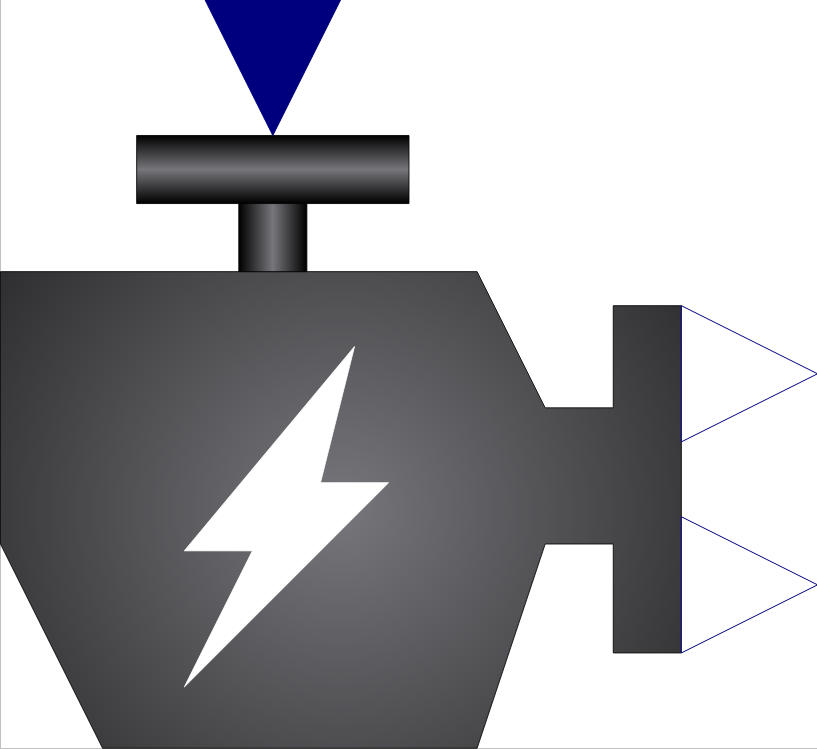
\includegraphics[width=0.15\textwidth]{Images/components/actuator}
\end{wrapfigure}

The Actuator model represents a standard linear actuator.
In addition to the configurable parameters described in \autoref{subsec:configuration}, the actuator features one input and two outputs: the input is setpoint\_motor, and the outputs are norm\_motor\_position and motor\_position.
Given a motor setpoint, the actuator adjusts its position over time to reach the desired value.
This motion is governed by two timing parameters: motor\_opening\_time and motor\_closing\_time.
When the actuator is at a given position and receives a new setpoint, it transitions to the new position at a rate proportional to these timing parameters.
Since the valve models expect the motor position to be normalized between 0 and 1, the input setpoint must be normalized using:

\[
setpoint_n = \frac{setpoint\_motor - min\_motor\_position}{max\_motor\_position - min\_motor\_position}
\]

From this normalized value, the actuator computes a new normalized motor position, norm\_motor\_position, which serves as the input to the valve models.
To recover the denormalized motor position, motor\_position, the following denormalization is applied:
\[
motor\_position = norm\_motor\_position \cdot (max\_motor\_position - min\_motor\_position) + min\_motor\_position
\]


\section{Valves}
\label{sec:valves}

\subsection{Linear Valve}
\label{subsec:linear-valve}

\begin{wrapfigure}{R}{0.15\textwidth}
    \centering
    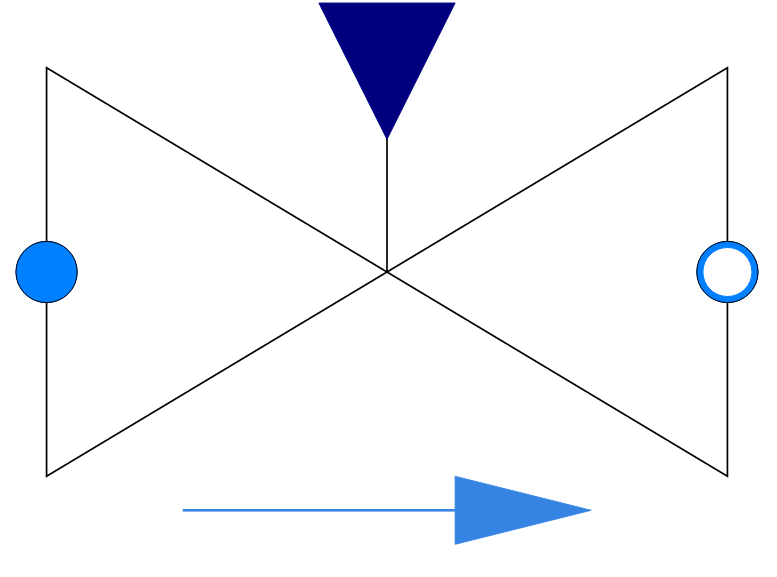
\includegraphics[width=0.15\textwidth]{Images/components/linear-valve}
\end{wrapfigure}

The LinearValve model serves primarly as a wrapper around the ValveIncompressible model from the Modelica.Fluid.Valves library.
This abstraction simplifies integration by pre-configuring all relevant parameters, allowing the linear valve to be easily added to flow models without additional setup.

In addition to the configurable parameters described in \autoref{subsec:configuration}, the linear valve features two inputs and one output: the inputs are motor\_position and port\_a, and the output is port\_b.
The motor\_position receives the normalized motor position from the actuator, port\_a and port\_b are the ends of the fluid connection constructing the flow path.

\newpage

\subsection{Equalpercentage Valve}
\label{subsec:equalpercentage-valve}

\begin{wrapfigure}{R}{0.15\textwidth}
    \centering
    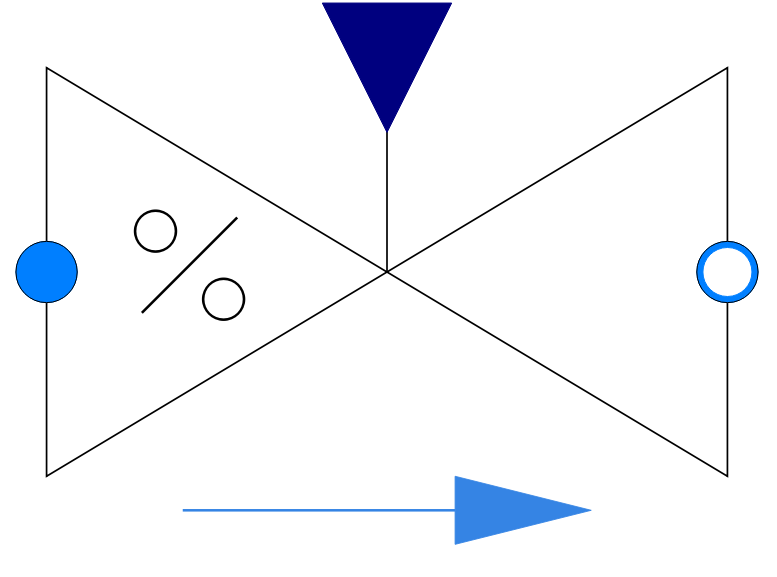
\includegraphics[width=0.15\textwidth]{Images/components/equi-valve}
\end{wrapfigure}

The EqualPercentageValve models serves primarily as wrapper around the TwoWayEqualPercentage model from the Buildings.Fluid.Actuators library.
This abstraction simplifies integration by pre-configuring all relevant parameters, allowing the equal percentage valve to be easily added to flow models without additional setup.

Similar to the linear valve, the equal percentage valve includes, in addition to the configurable parameters described in \autoref{subsec:configuration}, two inputs and one output.
The inputs are motor\_position and port\_a, while the output is port\_b.
The motor\_position receives the normalized motor position from the actuator, port\_a and port\_b are the ends of the fluid connection constructing the flow path.

\section{Pumps}
\label{sec:pumps}

\subsection{Pressure Pump}
\label{subsec:pressure-pump}

\begin{wrapfigure}{R}{0.15\textwidth}
    \centering
    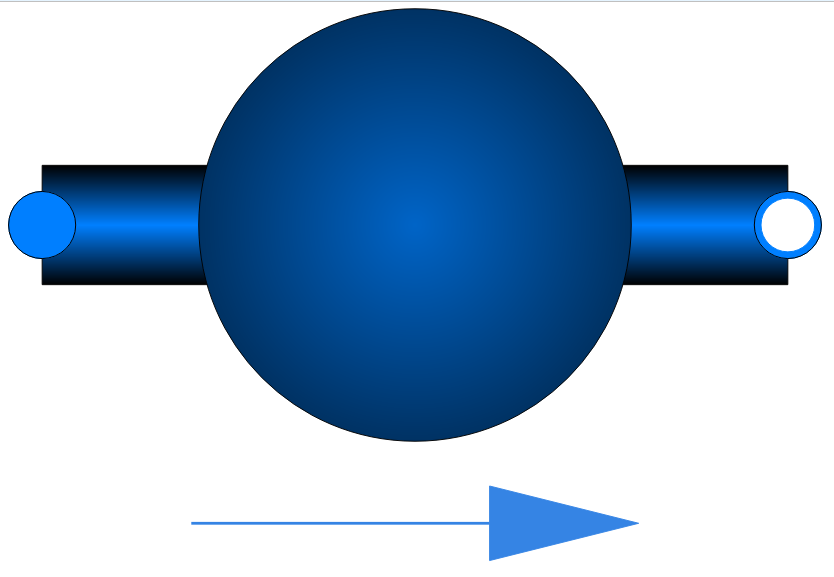
\includegraphics[width=0.15\textwidth]{Images/components/pressure-pump}
\end{wrapfigure}

The PressurePump model serves also primarily as a wrapper around the FlowControlled\_dp model from the Buildings.Fluid.Movers library.
This abstraction simplifies integration by pre-configuring all relevant parameters, allowing the pressure pump to be easily added to flow models without additional setup.

In addition to the configurable parameters described in \autoref{subsec:configuration}, the pressure pump features one input and one output: the input is port\_a, and the output is port\_b.
These are the ends of the fluid connection constructing the flow path.


\section{Sensors}
\label{sec:sensors}

\subsection{Flow Sensor}
\label{subsec:flow-sensor}

\begin{wrapfigure}{R}{0.15\textwidth}
    \centering
    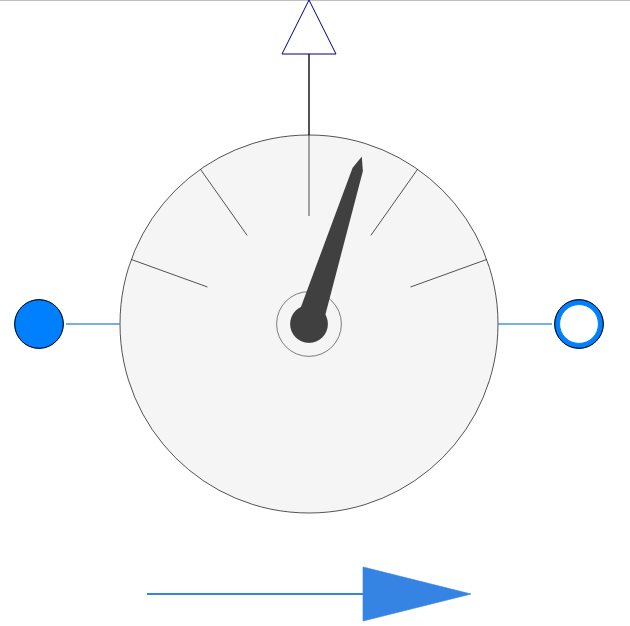
\includegraphics[width=0.15\textwidth]{Images/components/flow-sensor}
\end{wrapfigure}

The FlowSensor model serves also primarily as a wrapper around the VolumeFlowRate model from the Modelica.Fluid.Sensors library.
This abstraction simplifies integration by pre-configuring all relevant parameters, allowing the flow sensor to be easily added to flow models without additional setup.

Furthermore, since the VolumeFlowRate model provides its output in cubic meters per second $(m^{3}/s)$, the value is multiplied by 3600 to convert it to cubic meters per hour $(m^3 /h)$.

The flow sensor has one input and two outputs: the input is port\_a, and the outputs are flow\_rate and port\_b.
The flow\_rate is the measured flow and port\_a and port\_b are the ends of the fluid connection constructing the flow path.

\section{Pipes}
\label{sec:pipes}

\subsection{Pipe}
\label{subsec:pipe}

\begin{wrapfigure}{R}{0.15\textwidth}
    \centering
    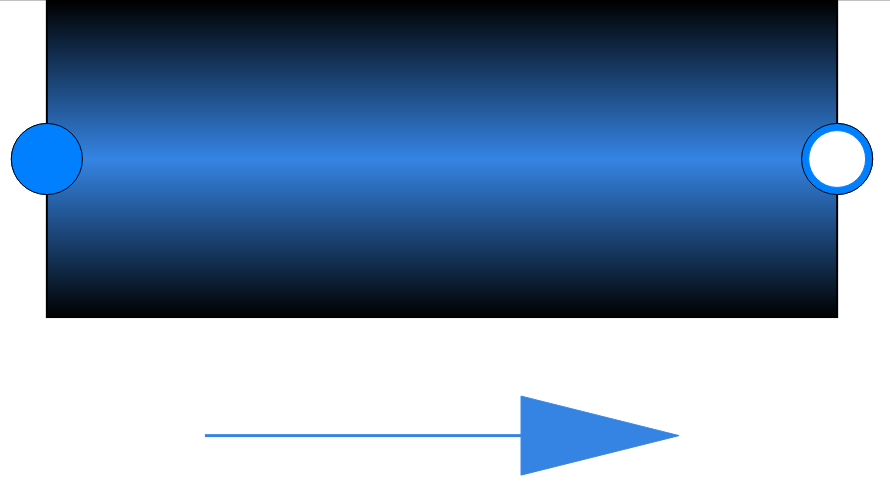
\includegraphics[width=0.15\textwidth]{Images/components/pipe}
\end{wrapfigure}

The Pipe model serves also primarily as a wrapper around the StaticPipe model from the Modelica.Fluid.Pipes library.
This abstraction simplifies integration by pre-configuring all relevant parameters, allowing the pipe to be easily added to flow models without additional setup.

Furthermore, when placing a pipe, a few parameters have to be set as shown in \autoref{tab:parameters-pipe}.
\begin{table}[h!]
    \centering
    \begin{tabular}{|lcl|}
        \hline
        \multicolumn{1}{|l|}{\textbf{Parameter}}     & \multicolumn{1}{c|}{\textbf{Unit}} & \textbf{Description}                                                                    \\ \hline
        \multicolumn{1}{|l|}{height}                 & \multicolumn{1}{c|}{mm}            & The length of the pipe                                                                  \\ \hline
        \multicolumn{1}{|l|}{diameter}               & \multicolumn{1}{c|}{mm}            & The diameter of the pipe                                                                \\ \hline
        \multicolumn{1}{|l|}{height\_ab}             & \multicolumn{1}{c|}{mm}            & The elevation of the pipe, such that $height\_ab = height_{port\_b} - height_{port\_a}$ \\ \hline
    \end{tabular}
    \caption{Parameters pipe}
    \label{tab:parameters-pipe}
\end{table}

The pipe has one input and one output: the input is port\_a, and the output is port\_b.
These are the ends of the fluid connection constructing the flow path.

\subsection{Bend}
\label{subsec:bend}

\begin{wrapfigure}{R}{0.15\textwidth}
    \centering
    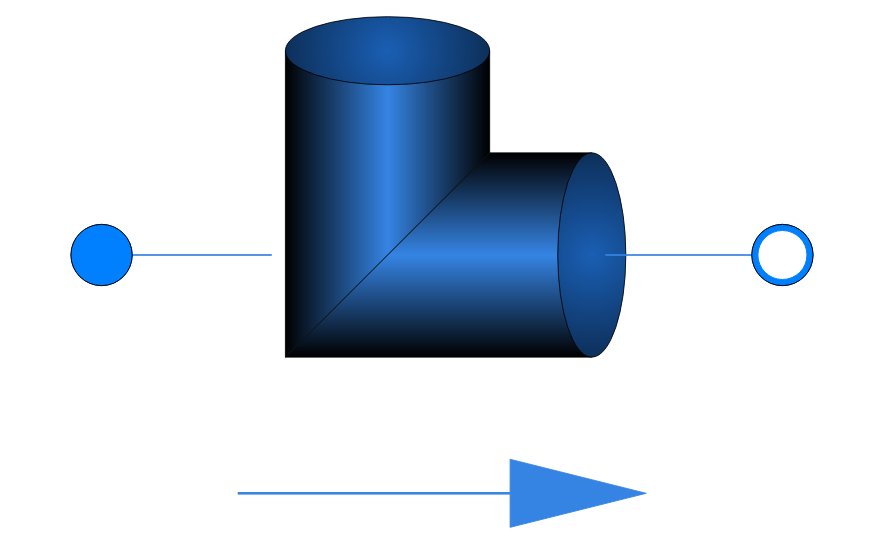
\includegraphics[width=0.15\textwidth]{Images/components/bend}
\end{wrapfigure}

The Bend model serves also primarily as a wrapper around the EdgedBend model from the Modelica.Fluid.Fittings.Bends library.

Furthermore, when placing a bend, a few parameters have to be set as shown in \autoref{tab:parameters-bend}.
\begin{table}[h!]
    \centering
    \begin{tabular}{|lcl|}
        \hline
        \multicolumn{1}{|l|}{\textbf{Parameter}}     & \multicolumn{1}{c|}{\textbf{Unit}} & \textbf{Description}     \\ \hline
        \multicolumn{1}{|l|}{angle}                  & \multicolumn{1}{c|}{degrees}       & The angle of the bend    \\ \hline
        \multicolumn{1}{|l|}{bend}                   & \multicolumn{1}{c|}{m}             & The diameter of the pipe \\ \hline
    \end{tabular}
    \caption{Parameters bend}
    \label{tab:parameters-bend}
\end{table}

The bend has one input and one output: the input is port\_a, and the output is port\_b.
These are the ends of the fluid connection constructing the flow path.

\newpage

\section{Dynamx}
\label{sec:dynamx}

\subsection{Linear Valve and Actuator}
\label{subsec:linear-valve-and-actuator}

\begin{wrapfigure}{R}{0.15\textwidth}
    \centering
    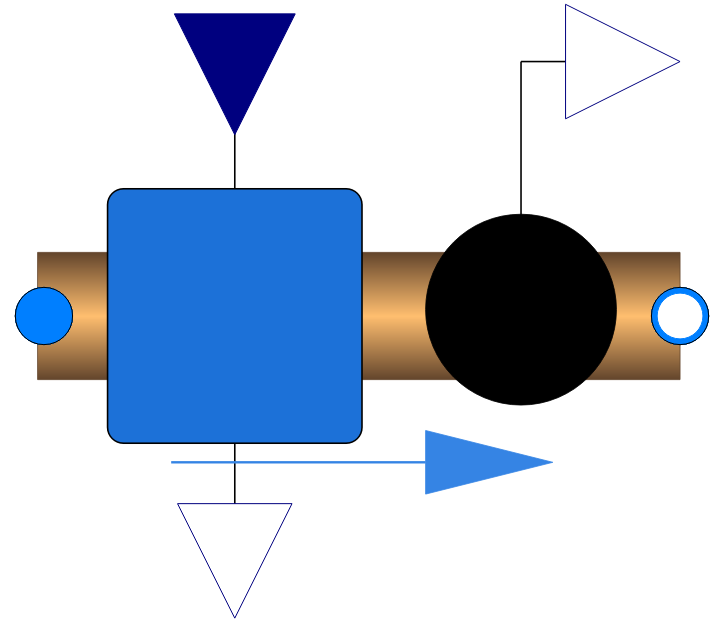
\includegraphics[width=0.15\textwidth]{Images/components/dynamx}
\end{wrapfigure}

The LinearDefaultActuator model combines the functionalities of the Actuator, LinearValve, and FlowSensor into a single Dynamx component.
This model extends the Components.BaseComponents.DynamxBase model.
To create a custom Dynamx model, it is recommended to also extend the Components.BaseComponents.DynamxBase model.
The parameters of a Dynamx model should be configured using the Configuration model.

In addition to the configurable parameters described in \autoref{subsec:configuration}, the dynamx models features two inputs and three outputs: the inputs are motor\_setpoint and port\_a, and the outputs are motor\_position, flow\_rate and port\_b.
The motor\_setpoint is the setpoint for the actuator, motor\_position is the calculated motor position by the actuator, flow\_rate is the measured flow rate by the flow sensor, and port\_a and port\_b are the ends of the fluid connection constructing the flow path.

\subsection{Equalpercentage Valve and Actuator}
\label{subsec:equalpercentage-valve-and-actuator}

The EqualPercentageDefaultActuator component is nearly identical to the LinearDefaultActuator, except that it uses the EqualPercentageValve instead of the LinearValve.

\section{Base Components}
\label{sec:base-components}

\subsection{Base Flow Model}
\label{subsec:base-flowmodel}

\begin{wrapfigure}{R}{0.15\textwidth}
    \centering
    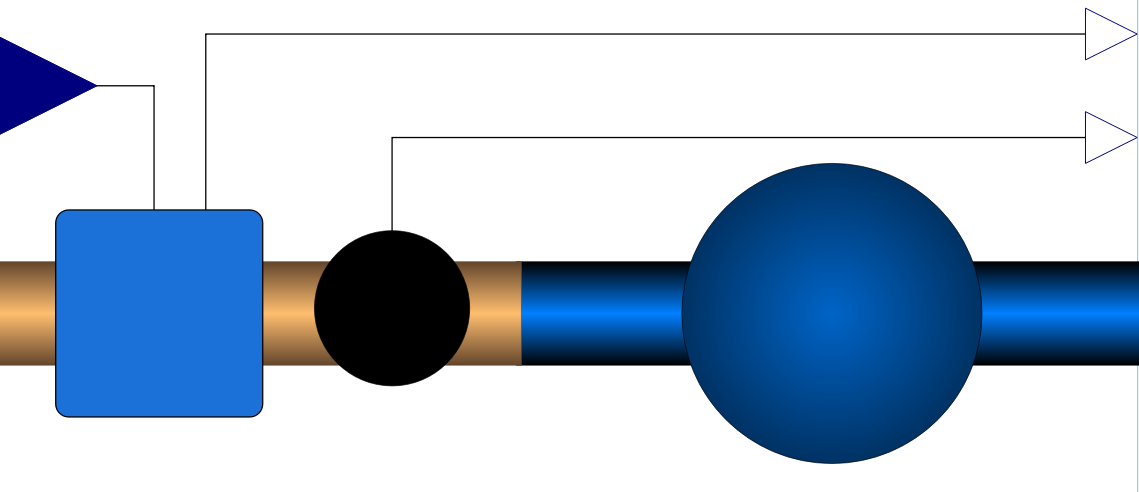
\includegraphics[width=0.15\textwidth]{Images/components/flow-model-base}
\end{wrapfigure}

When creating a new flow model, it is recommended to extend it from FlowModelBase.
This base model automatically provides all required inputs, outputs, and the configuration model with the correct predefined names.

By doing so, naming errors and missing interfaces or components are avoided.
Consistent naming is essential because the Python interface relies on specific names to locate inputs, outputs, and components within the model.

\subsection{Base Dynamx}
\label{subsec:base-dynamx}

\begin{wrapfigure}{R}{0.15\textwidth}
    \centering
    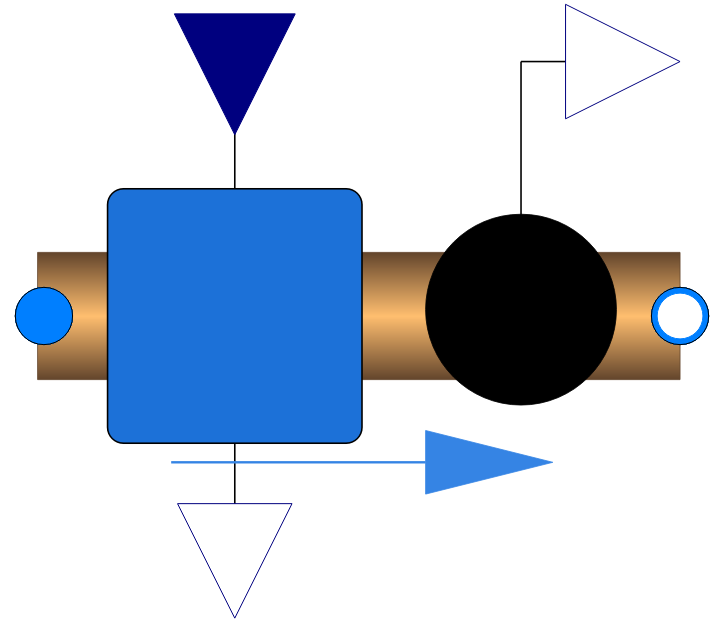
\includegraphics[width=0.15\textwidth]{Images/components/dynamx}
\end{wrapfigure}

All Dynamx models should extend this base model.
Similar to \texttt{FlowModelBase}, it automatically provides all required inputs and outputs.
In addition, a flow sensor is already included in the base model.

As a result, when creating a new Dynamx model, the user only needs to add a valve and an actuator.
Currently, all possible combinations of valves and actuators are already provided.
However, if new actuators or valves with different characteristics are introduced in the future, new Dynamx components can be easily created by extending this base model.

\subsection{Base Pipe Networks}
\label{subsec:base-pipe-networks}

\begin{wrapfigure}{R}{0.15\textwidth}
    \centering
    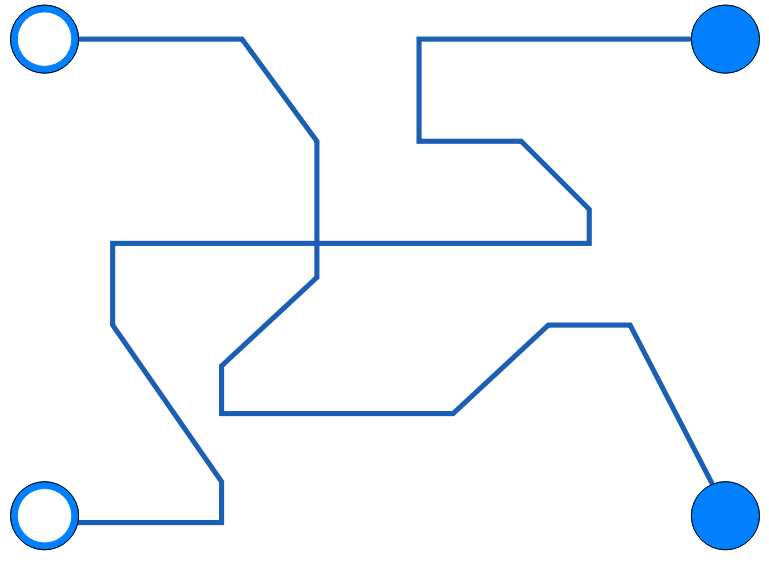
\includegraphics[width=0.15\textwidth]{Images/components/pipe-network}
\end{wrapfigure}

The final relevant base component is PipeNetworkBase.
When constructing a new network of pipes and bends, it should be extended from this component.
The PipeNetworkBase provides two inputs (input\_pump and input\_valve) and two outputs (output\_pump and output\_valve).

These connections are defined such that input\_pump links to port\_a of the pump and output\_pump to port\_b of the pump, with analogous connections for the valve.
This design ensures that the overall flow model consists of only three main components: a pipe network, a pressure pump, and a Dynamx component.

With this structure, modifying the pipe network requires changes only to the pipe network model itself—no outer connections need to be altered.
An example showing the connection between the pipe network, pressure pump, and Dynamx component is provided in \autoref{fig:example-pipe-network-connection}.

\begin{figure}[h!]
    \centering
    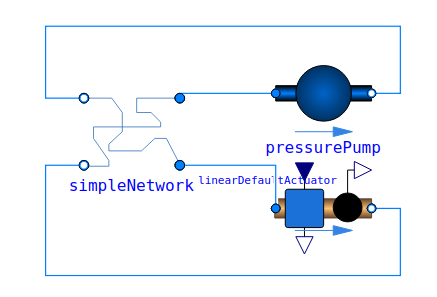
\includegraphics[width=0.4\linewidth]{Images/components/example_connection_pipe_network}
    \caption{Example connection between pipe network, pressure pump and Dynamx component}
    \label{fig:example-pipe-network-connection}
\end{figure}


\section{Pipe Networks}
\label{sec:pipe-networks}

\subsection{Simple Network}
\label{subsec:simple-network}

\begin{wrapfigure}{R}{0.15\textwidth}
    \centering
    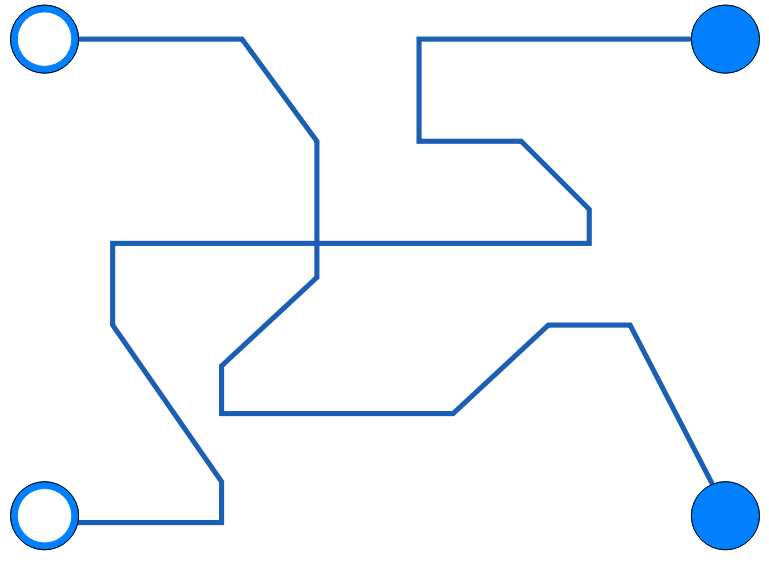
\includegraphics[width=0.15\textwidth]{Images/components/pipe-network}
\end{wrapfigure}

As an example of a pipe network, a simple reference model has been created to illustrate how the flow connections should be made.
This network contains a single pipe, where output\_valve is connected to port\_a of the pipe, and port\_b is connected to input\_pump.
Additionally, output\_pump is directly connected to input\_valve.

This configuration results in the following connection sequence: dynamx $\rightarrow$ pipe $\rightarrow$ pressure pump $\rightarrow$ dynamx.

% %%%%%%%%%%%%%%%%%%%%%%%%%%%%%%%%%%%%%%%%%%%%%%%%%%%%%%%%%%% %
% %%%%%%%%%%%%%%%%%%%%%%%%%%%%%%%%%%%%%%%%%%%%%%%%%%%%%%%%%%% %
% %%%%%%%%%%%%%%%%%%%%%%%%%%%%%%%%%%%%%%%%%%%%%%%%%%%%%%%%%%% %
\chapter{Python Interface}
\label{ch:python-interface}

The Python interface is centered around a main orchestrator class, Simulation, as described in \autoref{sec:complete-integration}.
In addition to this main class, the interface contains three subcomponents: FSBMock, Modbus, and Model.
\begin{itemize}
    \item The FSBMock class handles the functionality of the FSB.
    \item The Modbus class manages all Modbus-related functionality.
    \item The Model class is responsible for all Modelica-related operations.
\end{itemize}

Each of these classes has a corresponding configuration dataclass: FSBConfig, ModbusConfig, and ModelConfig.
While could not specify the configuration the Modbus due some privacy regelations \todo{Ask this, maybe it doesn't matter that much}, the ModelConfig and FSBConfig dataclass are described in detail.

The ModelConfig dataclass contains the following fields:
\begin{lstlisting}[style=pythonstyle, caption={ModelConfig data fields}]
@dataclass
class ModelConfig:
    fmu_path: str
    start_time: float
    stop_time: float
    step_size: float
    min_motor_position: int
    max_motor_position: int
    start_motor_position: int
    total_opening_time: int
    total_closing_time: int
    pump_pressure: float
    valve_diameter: int
    max_valve_flow_rate: float
\end{lstlisting}

All fields except the first four correspond to the parameters defined in the Modelica Configuration model, as listed in \autoref{tab:config-table}.
The first four fields are specific to the simulation setup:
\begin{itemize}
    \item fmu\_path: the file path to the FMU of the flow model.
    \item start\_time: the simulation start time.
    \item stop\_time: the simulation stop time.
    \item step\_size: the time increment for each simulation step.
\end{itemize}

These fields allow the Python interface to fully define and control the simulation while mapping the relevant Modelica parameters through ModelConfig.

The FSBConfig dataclass contains the following fields:

\begin{lstlisting}[style=pythonstyle, caption={FSBConfig data fields}]
@dataclass
class FSBConfig:
    port: str
    flow_send_rate: float
\end{lstlisting}

The port of the FSBConfig corresponds to the port used for the UART connection, as discussed in \autoref{sec:interaction-with-the-control-loop}.
The flow\_send\_rate is utilized in the simulation loop.
In the real-world application, the control loop expects a measurement from the FSB every x seconds.
To accurately test the control loop, the simulation must send a measurement at the same interval.
The detailed mechanism of this process is explained in Section \autoref{sec:complete-integration-extended}.
By using such a send rate, the simulation mirrors the timing of a real-life test case, ensuring realistic interaction with the control loop.

\section{Complete Integration Extended}
\label{sec:complete-integration-extended}

Now that we have implemented additional components in Modelica and aim for our simulation to reflect real-world behavior, it is necessary to extend the simulation loop to make it suitable for performing test simulations.

\begin{lstlisting}[style=pythonstyle, caption={Extended simulation loop}]
def run(self, setpoints: list[Tuple[float, float]]):
    performed_step = True
    p_bar = tqdm(total=self._total_iters, desc="Simulation Progress")
    s_flow = self._model.get_measured_flow()
    while performed_step:
        p_bar.update(1)
        # Update measured flow
        m_flow = self._model.get_measured_flow()
        self._fsb.update_flow(m_flow)
        # Update setpoint flow
        time = self._model.current_time
        new_s_flow, setpoints = self._get_setpoint_flow(setpoints, time)
        if new_s_flow:
            s_flow = new_s_flow
            self._modbus.set_setpoint_flow(s_flow)
        # Update setpoint motor
        s_motor = self._modbus.get_setpoint_motor()
        self._model.set_setpoint_motor(s_motor)
        # Retrieve motor position
        motor_pos = self._model.get_motor_position()
        # Update the trace
        self._update_trace(time, m_flow, motor_pos, s_flow, s_motor)
        # Perform a step
        performed_step = self._model.perform_step()
        # If operations are faster than the sample rate of the fsb, wait
        self._fsb.tick()
    p_bar.close()

--- Example input:
sim = Simulation(fsb_config, modbus_config, model_config)
setpoints = [(0.0, 1.0), (200.0, 1.5)]
sim.run(setpoints)
\end{lstlisting}

This extended simulation loop introduces several enhancements:
\begin{itemize}
    \item Setpoint input: Unlike the basic simulation loop, this version accepts a list of setpoints. As illustrated in \autoref{fig:full-communication-extended}, the User/Client system can provide new setpoints to the Modbus interface. Each tuple in the list contains a timestamp (first element) and the corresponding target setpoint for the actuator (second element).
    \item Progress bar: Since the simulation may take significant time, a progress bar is included to monitor simulation progress conveniently.
    \item Actuator position tracing: The Modelica model now returns the current actuator position. This position is retrieved in each loop iteration and added to the simulation trace, enhancing observability.
    \item FSB tick function: The tick function ensures that each loop iteration takes exactly the time specified by the flow\_send\_rate in FSBConfig. Performance testing showed that a single simulation step takes approximately 5 ms on average, while the intended send rate is 250 ms, leaving ample margin. For more complex flow models, loop execution time may increase; therefore, it is recommended to perform additional performance testing when creating new models. This can be done by temporarily disabling the tick function to measure the average loop execution time.
\end{itemize}

\begin{figure}[h!]
    \centering
    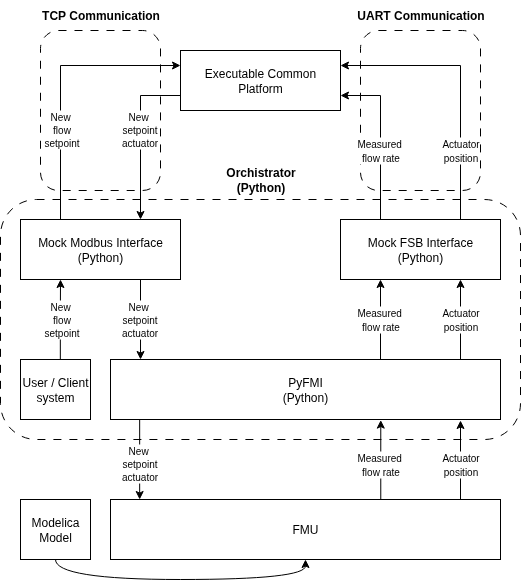
\includegraphics[width=0.6\linewidth]{Images/generated/full-communication-extended}
    \caption{Total interaction overview between all components extended}
    \label{fig:full-communication-extended}
\end{figure}

% %%%%%%%%%%%%%%%%%%%%%%%%%%%%%%%%%%%%%%%%%%%%%%%%%%%%%%%%%%% %
% %%%%%%%%%%%%%%%%%%%%%%%%%%%%%%%%%%%%%%%%%%%%%%%%%%%%%%%%%%% %
% %%%%%%%%%%%%%%%%%%%%%%%%%%%%%%%%%%%%%%%%%%%%%%%%%%%%%%%%%%% %
\chapter{Simulation Setup}
\label{ch:simulation-setup}

\section{Flow Models}
\label{sec:flow-models}

\section{Python Configurations}
\label{sec:python-configurations}

% %%%%%%%%%%%%%%%%%%%%%%%%%%%%%%%%%%%%%%%%%%%%%%%%%%%%%%%%%%% %
% %%%%%%%%%%%%%%%%%%%%%%%%%%%%%%%%%%%%%%%%%%%%%%%%%%%%%%%%%%% %
% %%%%%%%%%%%%%%%%%%%%%%%%%%%%%%%%%%%%%%%%%%%%%%%%%%%%%%%%%%% %
\chapter{Results}
\label{ch:results}

% %%%%%%%%%%%%%%%%%%%%%%%%%%%%%%%%%%%%%%%%%%%%%%%%%%%%%%%%%%% %
% %%%%%%%%%%%%%%%%%%%%%%%%%%%%%%%%%%%%%%%%%%%%%%%%%%%%%%%%%%% %
% %%%%%%%%%%%%%%%%%%%%%%%%%%%%%%%%%%%%%%%%%%%%%%%%%%%%%%%%%%% %
\chapter{Conclussion}
\label{ch:conclussion}

% %%%%%%%%%%%%%%%%%%%%%%%%%%%%%%%%%%%%%%%%%%%%%%%%%%%%%%%%%%% %
% %%%%%%%%%%%%%%%%%%%%%%%%%%%%%%%%%%%%%%%%%%%%%%%%%%%%%%%%%%% %
% %%%%%%%%%%%%%%%%%%%%%%%%%%%%%%%%%%%%%%%%%%%%%%%%%%%%%%%%%%% %
\appendix

\bibliographystyle{plain}
\bibliography{refs}

\end{document}
